\chapter{Preliminaries}
\label{chapter:preliminaries}

In this chapter we introduce the RoboTour competition,
discuss several basic techniques of image segmentation,
describe the functionality and inner workings of convolutional neural network (CNN) as well as 
its impact on image segmentation. The chapter also includes description of layers relevant
for CNNs applied to semantic segmentation.

\section{RoboTour competition}
\label{sec:robotour}

RoboTour Outdoor Delivery Contest is an annual competition for outdoor robots being held
in different locations, which are mostly parks.
The participants are challenged to build an autonomous robot which completes the task
without breaking rules. The robot starts at the position $A$
(also called the base, where it is possible to repair or calibrate the robot) and
is given GPS coordinates of position $B$. Then, the robot must navigate itself through
the park to the location $B$ where organizers of the competition load a five liter
barrel of beer onto it. The robot is once again given coordinates, but this time
of position $C$
where it is supposed to deliver the barrel. After unloading, the final goal is to return
back to the base.

\begin{figure}[!h]
	\centerline{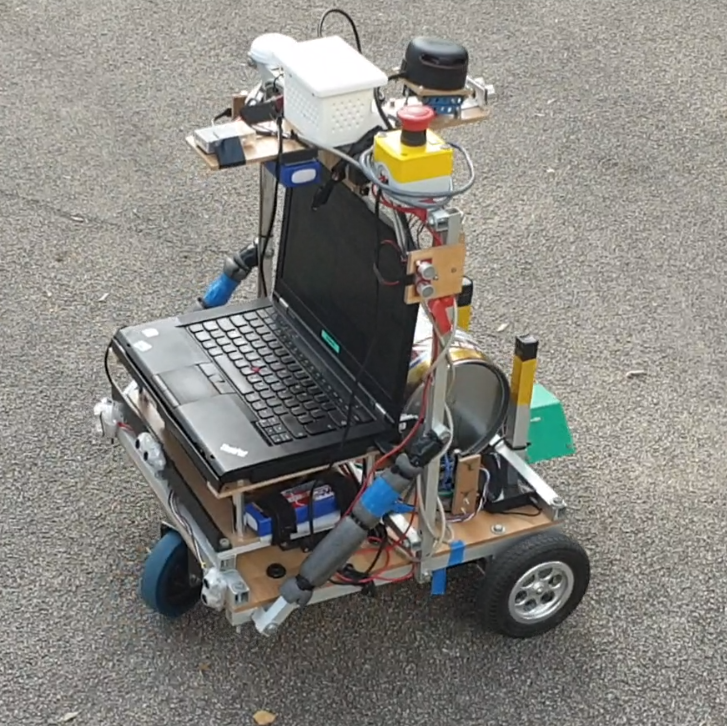
\includegraphics[width=0.5\textwidth]{images/zajkophoto.png}}
	\caption[The photo of our robot Smelý Zajko]{The photo of our robot Smelý Zajko, heading to delivery point in Deggendorf.}
	\label{img:zajko}
\end{figure}

The robot is forbidden both to leave the driveable path or to touch any obstacle during
the round. If such event occurs, the robot is immediately disqualified from the round.
Therefore, it is important for the robot to prevent breaking the rules. Avoiding
obstacles is done quite accurately using laser and ultrasonic sensors mounted on the
robot. Our robot (see Figure \ref{img:zajko})
is also equipped with camera for local navigation so it tries not to leave the road.
In this work we focus on the problem of differentiating between two categories within
given image (driveable or non-driveable path) using computer vision technique called
convolutional neural networks solving semantic segmentation.

\section{Image segmentation}
\label{sec:image_segmentation}

Extracting useful information from images is an inevitable step for image analysis.
Image segmentation is a computer vision task of automatic image analysis.
Its main task is to partition an image into multiple
classes and extract objects or regions of interest from background.
Each pixel within this image is assigned a class or a category which
it belongs to. Pixels with the same label share certain characteristics.
\cite{bib:zhang2009image}

The history of image segmentation can be traced back to 50 years ago.
Since then, many techniques have been developed and evaluated.
We are going to describe some of them.
One of them is a machine learning technique that utilizes convolutional neural networks
(CNNs), which we will describe in the Section \ref{sec:cnn}.

\subsection{Region-based segmentation}
\label{sec:image_segmentation:region_based}

\subsubsection{Threshold segmentation}
\label{sec:image_segmentation:region_based:threshold}

Threshold segmentation is one of the most commonly used and simplest techniques.
The input image is transformed into grayscale representation. Global and local threshold
methods can be used afterwards. The former uses just one global threshold
value and divides the image into just two regions - target and background. On the other
hand, local threshold method uses multiple threshold values to divide the image
into multiple target and background regions.

Simple calculations make this method very fast. If the contrast between
background and the target is high enough, the segmentation can be computed quite
accurately. The disadvantage of this method is that it is difficult to obtain
accurate results where there is no significant difference in grayscale image, since
it does not take the spatial information into account. \cite{bib:yuheng2017image}

\subsubsection{Regional growth segmentation}
\label{sec:image_segmentation:region_based:reggrowth}

The basic idea of regional growth segmentation method is to merge neighboring
pixels (or regions) that share similar properties into one. The first step
is to select so called seed pixels. We then grow regions from them, merging pixels
if their absolute difference is less or equal to some threshold $T$.
Visiting input pixels is done by breadth-first search.

The main disadvantages of the aforementioned method are that it is computationally expensive
local method with no global view and it is quite sensitive to noise .

In the Figure \ref{img:regionalgrowthexample},
there is an example of the algorithm starting with input (leftmost) matrix. The middle
matrix is computed using threshold $T=3$ and the second one using $T=6$. We can clearly
see that the choice of the threshold value is very important step for this algorithm
to work properly. \cite{bib:yuheng2017image}

\begin{figure}[!h]
    $$\begin{bmatrix}
    \textbf{1} & 0 & 4 & 7 & \textbf{5} \\
    1 & 0 & 5 & 7 & 7 \\
    0 & 1 & 5 & 5 & 5 \\
    2 & 0 & 5 & 6 & 5 \\
    2 & 2 & 5 & 6 & 4
    \end{bmatrix}
    \hspace{2cm}
    \begin{bmatrix}
    1 & 1 & 5 & 5 & 5 \\
    1 & 1 & 5 & 5 & 5 \\
    1 & 1 & 5 & 5 & 5 \\
    1 & 1 & 5 & 5 & 5 \\
    1 & 1 & 5 & 5 & 5
    \end{bmatrix}
    \hspace{2cm}
    \begin{bmatrix}
    1 & 1 & 1 & 1 & 1 \\
    1 & 1 & 1 & 1 & 1 \\
    1 & 1 & 1 & 1 & 1 \\
    1 & 1 & 1 & 1 & 1 \\
    1 & 1 & 1 & 1 & 1
    \end{bmatrix}
    $$
    \caption[Example of regional growth segmentation]{Example of regional growth segmentation.}
    \label{img:regionalgrowthexample}
\end{figure}

\subsection{Edge detection segmentation}
\label{sec:image_segmentation:edge_based}

Edges represent the most significant changes in the image. That includes changes in
brightness, colors, etc. This method involves detection of abrupt pixel discontinuities
and arranges them into edges (for example transition from one color to another).
\cite{bib:yuheng2017image}

\subsection{Clustering-based segmentation}
\label{sec:image_segmentation:cluster_based}

Clustering is widely known as a method of iterating over samples in a feature space
and computing the nearest cluster they belong to. After convergence of pixels,
we can map them back to the original image to get the segmentation results.

The most frequently used clustering algorithm is K-means. It consists of four steps:

\begin{enumerate}
	\item Initialize clusters - select random samples to be centroids of the cluster
	\item Assign each sample to cluster - calculate the distance from each cluster and
	assign the sample to the nearest one
	\item Recompute the centroid of each cluster by taking the mean of its samples
	\item Repeat steps 2 and 3 until none of the samples changes the cluster
\end{enumerate}

The K-means algorithm is fast and easy to implement and scalable to large
datasets. Unfortunately, the parameter $K$ (the number of clusters)
is difficult to estimate and has to be chosen experimentally.
As the authors of \cite{bib:yuheng2017image} mention, it is distance-based partitioning method and
therefore it is only applicable to convex datasets.

\subsection{Histogram-based segmentation}
\label{sec:image_segmentation:histogram_based}

Histogram-based segmentation is a very efficient method in terms of computation since
it only requires one pass through the image. During that pass it computes histogram
from the pixels. The histogram peaks are then used to locate objects within the image.
This method can be improved by recursively applying it to clusters in order to divide
them into smaller ones. One disadvantage of histogram-based segmentation is that
it might be difficult to identify significant peaks.

\section{Neural networks}
\label{sec:nn}

\begin{figure}[!h]
	\centerline{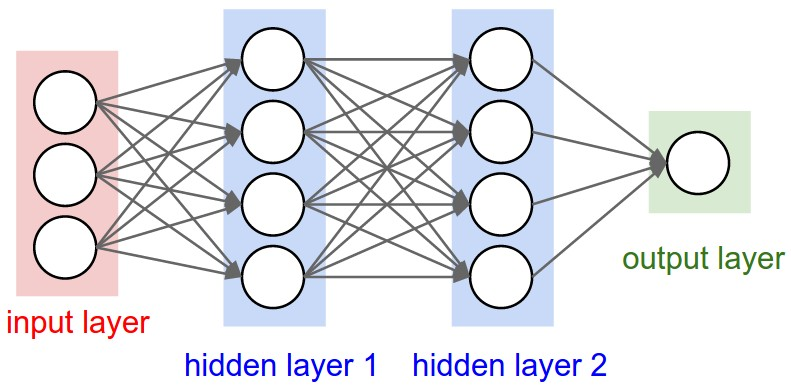
\includegraphics[width=0.5\textwidth]{images/neural_net.jpeg}}
	\caption[Multi-layer perceptron]{Multi-layer perceptron. (Image taken from \cite{bib:cnncs231n})}
	\label{img:neural_net}
\end{figure}

The development of neural networks has been primarily inspired by the goal of
modeling biological neural systems, but has diverged and become the matter of engineering.
These networks have been adopted to a wide range of tasks while beating previous
state-of-the-art techniques. The basic unit of the brain is neuron and has been
mathematically defined. In the late 1950s, Frak Rosenblatt developed the so called perceptron
for classifying objects. It takes a vector $\Vec{x}$ as the input, multiplies it
with weight vector $\Vec{w}$ and sums the resulting product. If this product is
above certain threshold, neuron fires and outputs the number 1, otherwise 0.
In the most common literature, there is a \textit{bias} term introduced and
responsible for shifting the decision boundary. The equation can be written
as $\sum_{i=1}^n x_iw_i + b$.

\textit{Multi-layer perceptron} (MLP) is the basic and probably the most widely
known feedforward artificial neural network. We can think of MLP as just a mathematical
function that maps inputs to output categories. It is formed by layers, which contain
several perceptrons accompanied by some nonlinearity (also reffered to as
\textit{activation function}), where each of this
neurons reads input from all of the neurons in previous layer. The standard MLP consists
of \textit{input} and \textit{output} layers, and several layers in between called
\textit{hidden} layers, see Figure \ref{img:neural_net}. \cite{bib:goodfellow2016deep}
Once we obtain the output from the network, we compute
the loss and the weights are then updated using backpropagation, see detailed description in
\cite{bib:goodfellow2016deep}.
The loss is a function denoting how much the predicted values differ from the ground truth. Furthermore,
it needs to be differentiable so we are able to compute direction in
multidimensional space which leads to update of the model's weights that improve our results.

\subsection{Activation functions}
\label{sec:nn:activation_functions}

As we mentioned in Section \ref{sec:nn}, neurons are accompanied by an activation function.
This is always some nonlinear function, since the linear function would not bring any
advantage and we could collapse all the layers into one. Let's have a look at some of
the most commonly used nonlinearities presented in Figure \ref{img:nonlinearities}.

\begin{figure}[h]
	\begin{center}
	    \subfloat[Sigmoid]{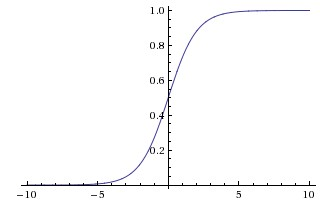
\includegraphics[width=0.32\textwidth]{images/sigmoid.jpeg}}
		\hspace{0.1em}
		\subfloat[Hyperbolic tangent]{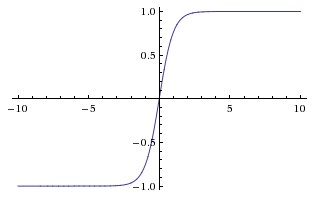
\includegraphics[width=0.32\textwidth]{images/tanh.jpeg}}
		\hspace{0.1em}
		\subfloat[ReLU]{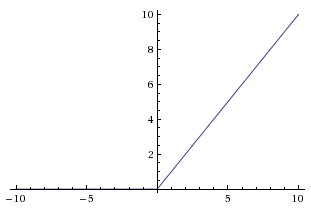
\includegraphics[width=0.32\textwidth]{images/relu.jpeg}}
	\end{center}
	\caption[Nonlinear functions]{Nonlinear functions.}
	\label{img:nonlinearities}
\end{figure}

\textit{Sigmoid} $\sigma(x) = \frac{1}{1+e^{-x}}$ takes real value number and squashes it
into a range between 0 and 1. Recently, sigmoid has fallen out of favor because it suffers
from saturation. If the neuron's activation saturates at either tail of 0 or 1, the gradient
at these regions is almost zero, which essentially stops the learning process. This phenomenon is called
\textit{vanishing gradient} in the literature \cite{bib:goodfellow2016deep}.

\textit{Tanh} $\textrm{tanh}(x) = 2\sigma(2x) - 1$ (hyperbolic tangent) activation is very
similar to the sigmoid. It also saturates, but on the other hand, its output is zero
centered. Note, that tanh is just a scaled sigmoid function.

\textit{ReLU} $\textrm{relu}(x) = \max(0, x)$ (rectified linear unit),
is another nonlinear activation function heavily used nowadays, mostly in computer
vision applications. It greatly accelerates the convergence of stochastic gradient
descent as found in \cite{bib:krizhevsky2012imagenet}. If we compare it to sigmoid or tanh
activations, ReLU is much easier to compute and can be implemented by thresholding a matrix
activations at zero. However, neurons with ReLU activation might die during training because
a large gradient could cause the weights to update in such a way that these neurons will
never activate and the gradient flowing through them will forever be zero. With the proper
setting of the learning rate, however, this is less frequently an issue. One may encounter other
variants of ReLU trying to fix this problem, such as \textit{Leaky ReLU}
\cite{bib:maas2013rectifier} or \textit{Parametric ReLU} \cite{bib:he2015delving}.
\cite{bib:cnncs231n}

\subsection{Learning concepts}
\label{sec:nn:learning_concepts}

There are three major learning concepts covering most of the contemporary machine learning:
\begin{enumerate}
    \item Supervised learning
    \item Unsupervised learning
    \item Reinforcement learning
\end{enumerate}

Supervised learning represents subset of machine learning techniques where the model
is provided with data along with ground truth labels. During training, the model makes
predictions, compares its results with the correct ones and adjusts parameters to
decrease the error.

Unsupervised learning stands for searching for patterns and similarities within dataset,
grouping similar ones together and detects anomalous samples. That means there are no ground
truth labels at all. Some popular examples of such models utilizing
unsupervised learning are \textit{K-means}, \textit{Self-organizing map} etc.

In reinforcement learning, there is an agent exploring some sort of environment being
rewarded for actions. Either positively or even negatively. The goal of the agent is to
observe the environment and learn underlying model to maximize the reward.
\cite{bib:sutton1998introduction}

In the convolutional neural network setting, applications usually make use of supervised
learning. In this work, our labels are ground truth masks - binary images of the same resolution
as input images, but each pixel being marked either as driveable (value 1) or non-driveable
(value 0).

%------------

\subsection{Parameter updates}
\label{sec:nn:parameter_updates}

Once we are training a neural network, we are evaluating our loss function.
Computing the gradient
of this function directs us towards updating the parameters in such a direction that
decreases the error computed by the loss function.
There are several approaches we can use for performing the update of parameters.
The most basic form of update is \textit{Gradient Descent}. After evaluating the loss function,
we can compute the negative gradient and update the parameters by the following formula
$$\theta = \theta - \alpha\nabla_{\theta} C(\theta)$$
where $\theta$ denotes the parameters, $\alpha$ denotes learning rate (fixed constant),
$C(\theta)$ is the loss function and $\nabla_{\theta} C(\theta)$ is gradient of the
loss function
with respect to $\theta$. Updating the parameters once after evaluating the entire dataset
becomes very inefficient in machine learning setting, especially when the dataset is very
large. The modification of this algorithm
performs the update after each training sample is evaluated and is called
\textit{Stochastic Gradient Descent} (SGD). However, it is a common practice nowadays to use
\textit{minibatch SGD} which essentially takes the average of gradients of small portion
of training examples and performs the parameter update accordingly.

In order to converge even faster, \textit{Momentum update} is another approach for
deep networks. It helps accelerate SGD in relevant direction and dampens oscillations.
The loss can be interpreted as hilly terrain and we push a ball down a hill. The ball
accumulates its velocity and is able to pass through slight hills in its way in order
not to end up in local minimum. The momentum technique modifies gradient descent
by introducing a new variable $v$ representing the velocity and a smoothing constant
$\beta$, which helps in controlling the value of $v$.
We can use the following formula to compute velocity in step $t$
$$v_t = \beta v_{t-1} - \alpha\nabla_{\theta} C(\theta)$$
and the parameters are updated by the velocity $\theta = \theta + v_t$.

\textit{Nesterov momentum}, based on Nesterov accelerated gradient
\cite{bib:nesterov1983convex}, has gained popularity for its stronger theoretical
convergence guaranty for convex functions. Moreover, it is in practice slightly better than
standard momentum. Its core idea is to look ahead, so our ball is smarter and knows
to slow down before the hill slopes up again. Computing $\theta + \beta v_{t-1}$
gives us an approximation of the next position of parameters. The revised velocity
update is
$$v_t = \beta v_{t-1} - \alpha\nabla_{\theta} C(\theta + \beta v_{t-1})$$
and the parameters update stays the same.

Previously discussed approaches manipulate the learning rate globally and equally for all
parameters. A lot of work has been put into methods that can adaptively tune the learning
rates, and even do so per parameter.
One of the most used method especially for convolutional neural networks is
\textit{Adam} (Adaptive Moment Estimation) \cite{bib:kingma2014adam}. The update of
the parameters is done by following formula:
$$m_t = \beta_1 m_{t-1}(1-\beta_1)\nabla_{\theta} C(\theta)$$
$$v_t = \beta_2 v_{t-1} + (1-\beta_2)\nabla_{\theta} C(\theta)^2$$
$$\theta = \theta - \alpha \frac{m_t}{\sqrt{v_t} + \epsilon}$$
where $\beta_1$ and $\beta_2$ denote decay rates. Authors suggest to set them to
$\beta_1 = 0.9$ and $\beta_2 = 0.999$.
The $\epsilon$ prevents from dividing by zero and is set to $\epsilon = 10^{-8}$.
The full Adam update also includes a bias correction mechanism, which tries to fix
that both $m$ and $v$ are in the beginning biased at zero. With the bias correction mechanism
the update looks as follows
$$\hat{m}_t = \frac{1}{1-{\beta_1}^t}$$
$$\hat{v}_t = \frac{1}{1-{\beta_2}^t}$$
$$\theta = \theta - \alpha \frac{\hat{m}_t}{\sqrt{v_t} + \epsilon}$$
There are also many other optimizers available. Sometimes, it is worth trying SGD
combined with Nesterov momentum as it might work slightly better in some cases.
\cite{bib:cnncs231n}

\section{Convolutional neural networks}
\label{sec:cnn}

Convolutional neural networks (CNNs or ConvNets) are a class of deep neural networks.
They are quite similar to ordinary neural networks, because they are made up of
neurons that have learnable weights and biases. By \textit{ordinary} we mean well known
multi-layer perceptron (MLP). CNNs are often applied to computer vision problems like
image classification, instance segmentation, semantic segmentation, object detection etc.

The CNN is a sequence of layers. It takes an image as the input, transforms
it layer by layer and outputs the final prediction. The CNN is given so called training data,
which are used during the training process. Each sample image
is fed into CNN and the output is compared to the ground truth and based on the result
both loss and accuracy functions are computed.

There should be also validation
data available which are often small portion of training data and network should never see them.
Their purpose is to see approximation of model's performance in real-world scenario and stop
training process in order to prevent overfitting.

We can clearly see from the results published that ConvNets are so powerful that they have
overcome classic computer vision techniques known before and are now
state-of-the-art in various areas.

Networks for semantic segmentation utilize an encoder network followed by a decoder network.
Encoder is usually a pre-trained model. Architectures mostly differ in their choice of the decoder.
The job of the encoder is to learn discriminative features at different stages and
encode them into high-dimensional feature
vector, whilst decoder takes this vector and produces semantic segmentation mask.
\cite{bib:semanticsegoveryears}

Every ConvNet architecture consists of several types of layers. Let's have a deeper
look on these building blocks in following subsections. 

\subsection{Fully-connected layer}
\label{sec:cnn:fclayer}

Fully-connected or FC layer has been adopted from the ordinary multi-layer perceptron.
Each neuron is connected to all the neurons from previous layer and fires activations to all
the neurons in following layer. Such layers are mostly located at the tail of ConvNet.
Features extracted by convolutional layers are fed into fully-connected ones which
firstly transform input into a single vector and then decide the class presence.

These layers usually contain most of the network's parameters and thus are a very expensive
part in terms of computation and model's size.
Most of the modern architectures doing semantic segmentation
avoid using fully-connected layers, resulting in more efficient models.

\subsection{Convolutional layer}
\label{sec:cnn:convlayer}

This type of layer is a core building block of a CNN.
Each one consists of a set of trainable filters with weights. These filters, also
called kernels,
are usually small spatially (along width and height) but extend through the full depth
of input volume. Each slice of depth channel can be referred to as a \textit{depth slice}. 
The number of filters corresponds to the depth of output volume.
For example, filters in the first layer might have size $5\times5\times3$
(5 pixels wide, 5 pixels high and depth 3, because our input image has 3 color
channels - red, green and blue). During the forward pass, we convolve (or slide) filter by filter through
the image and compute dot product at each region.
Denoting filter's weights $W_{w,h,d}$ and particular image region $R_{w,h,d}$ where
$w$ is width, $h$ is height, $d$ is depth and $b$ is a bias, we can compute
their dot product by the following formula
$$y_{i,j} = b + \sum_{i=1}^{w}\sum_{j=1}^{h}\sum_{k=1}^{d}w_{i,j,k}\cdot r_{i,j,k}$$

Each filter produces a 2D activation map $Y_{i,j}$.
These maps are then stacked along the depth dimension and passed as the input volume for
activation.
Intuitively, ConvNets learn filters that activate when they see specific feature such
as an edge, color and so on. Typically, in standard multi-layer perceptron
neural networks, each neuron
receives input from all of the neurons from previous layer. In ConvNets, each neuron
receives input only from restricted region from input volume. This region is defined
by aforementioned filter size, also referred to as \textit{receptive field}.

Authors of ConvNet architectures sometimes make use of $1\times 1$ convolutions.
This might sound
a bit confusing, but recall that filters extend through the full depth of input volume.
Therefore, we are able to control the depth of output volume by creating a layer with several
$1\times 1$ filters.

The basic convolutionalization downsamples the image spatially since dot product is not
defined for border pixels. This is undesirable behaviour in most cases. To keep width
and height dimensions of input and output volumes equal, we have to apply \textit{padding}
operation beforehand. The idea is to add enough zeros around the image borders.

\begin{figure}[!h]
    \centering
    \begin{tabular}{|r|r|r|r|r|}
        \hline
        \textbf{0} & \textbf{0} & \textbf{0} & \textbf{0} & \textbf{0} \\ \hline
        \textbf{0} & \multicolumn{3}{c|}{\multirow{3}{*}{image}} & \textbf{0} \\ \cline{1-1} \cline{5-5} 
        \textbf{0} & \multicolumn{3}{c|}{}                  & \textbf{0} \\ \cline{1-1} \cline{5-5} 
        \textbf{0} & \multicolumn{3}{c|}{}                  & \textbf{0} \\ \hline
        \textbf{0} & \textbf{0} & \textbf{0} & \textbf{0} & \textbf{0} \\ \hline
    \end{tabular}
    \caption[Padding image with zeros]{Padding image with zeros. Padding with one 0 on each side
    is usually done before applying $3\times 3$ filter. For $5\times 5$ we pad the image
    with two 0s and for $7\times 7$ with three 0s.}
    \label{img:zeropadding}
\end{figure}

On the other hand, we might sometimes need to downsample the image via ConvNet layer. The
output's volume size can also be controlled by \textit{stride} hyperparameter. Stride is
the number of steps we make to shift the filter to next region. In practice, if we want
to reduce the output size by convolutional layer, stride is mostly set to $2$
(uncommonly 3). When the stride is set to $1$, we move the sliding window one pixel at a
time.

To summarize the convolutional layer: \cite{bib:cnncs231n}
\begin{itemize}
    \item accepts input of size $W_1\times H_1 \times D_1$
    \item sets hyperparameters \textbf{\textit{K}} (number of filters),
        \textbf{\textit{F}} (filter's size), \textbf{\textit{S}} (stride) and
        \textbf{\textit{P}} (amount of zero padding)
    \item produces output of size $W_2\times H_2\times D_2$ where:
    \begin{itemize}
        \item[$\square$] $W_2 = (W_1 - F + 2P) / S + 1$
        \item[$\square$] $H_2 = (H_1 - F + 2P) / S + 1$
        \item[$\square$] $D_2 = K$
    \end{itemize}
\end{itemize}

\subsection{Pooling layer}
\label{sec:cnn:poollayer}

The common practice in ConvNets architectures is to use \textit{pooling layer} in between
convolutional layers. The purpose of the pooling layers is to achieve spatial invariance
by reducing the resolution of the feature maps 
which in the end leads to dramatic reduction of computing power, memory consumption and also
control of overfitting.

\begin{figure}[!h]
    \centering
    \begin{tabular}{p{2.3cm}p{3cm}}
        \begin{minipage}{.5\linewidth}
            \begin{tabular}{|l|l||l|l|}
                    \hline
                    1 & 4 & 2 & 2 \\ \hline
                    3 & 5 & 7 & 9 \\ \hline \hline
                    1 & 1 & 1 & 4 \\ \hline
                    0 & 1 & 7 & 2 \\ \hline
                \end{tabular}
        \end{minipage} &
        $\Rightarrow$
        \begin{minipage}{.5\linewidth}
            \begin{tabular}{|l||l|}
                    \hline
                    5 & 9  \\ \hline \hline
                    1 & 7  \\ \hline
                \end{tabular}
        \end{minipage} 
    \end{tabular}
    \caption[Max pooling example]{Max pooling example.}
    \label{img:maxpooling}
\end{figure}

Each depth slice is processed individually and therefore depth of the volume remains
unchanged. Similarly to the convolutional layer, it contains the sliding window, but this time
we are not computing dot product. The window takes values from the input volume's region
and computes a
simple function like \textit{max}
(called \textit{max pooling}, see Figure \ref{img:maxpooling}) or \textit{average}
(called \textit{average pooling}). In practice, it has been shown that max pooling performs
better than average pooling \cite{bib:scherer2010evaluation}.
Most widely used pooling layer is $2\times 2$ with a stride of
2, which reduces both width and height by a factor of 2. We may sometimes encounter
$3\times 3$ pooling layers with a stride of 2 (also called \textit{overlapping})
being used in ConvNet architectures, but in general there is
no significant improvement over using non-overlapping ones.
\cite{bib:cnncs231n, bib:scherer2010evaluation}\\


\subsection{Upsampling layers}
\label{sec:cnn:upsampling_layers}

The upsampling technique has been mostly used in semantic segmentation architectures.
When we input an image to the ConvNet, an encoder takes care of downsampling the image
to the very low resolution and classifying all the pixels. The decoder's role is to
upsample this output to the original size while preserving as much information as possible.
There are more ways to upsample the image. In the following subsections we describe
two of them, namely \textit{Unpooling} and \textit{Transposed convolution}.

\subsubsection{Unpooling layer}
\label{sec:cnn:upsampling_layers:unpooling_layer}

Unpooling is a simple upsampling layer with no trainable parameters. In practice,
the pooling operation is non-invertible, but we can approximate this inversion 
using unpooling layer. For example, many architectures
remember indices of maxima within each region when doing max-pooling and reuse them
to fill appropriate region. The rest of the grid is usually filled with zeros, see Figure
\ref{img:poolingindices}.
The most common unpooling layer with kernel size of $2\times 2$ upsamples
input of size $n\times n$ to $2n\times 2n$. \cite{bib:zeiler2014visualizing}

\begin{figure}[!h]
	\centerline{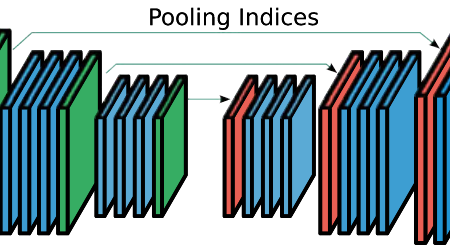
\includegraphics[width=0.35\textwidth]{images/pooling_indices2.png}
	    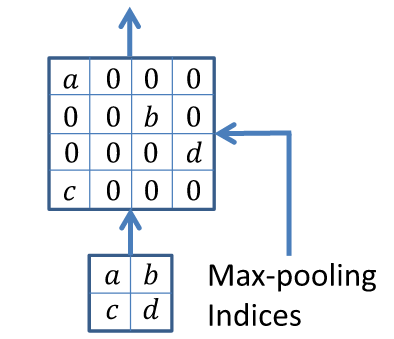
\includegraphics[width=0.35\textwidth]{images/pooling_indices.png}}
	\caption[Demonstration of how pooling indices are reused]{Demonstration of how pooling indices are reused in the decoder part. (Image taken from \cite{bib:szegedy2015going})}
	\label{img:poolingindices}
\end{figure}

\subsubsection{Transposed convolutional layer}
\label{sec:cnn:upsampling_layers:deconv_layer}

Transposed convolution (also called fractionally-strided convolution)
is a layer used for upsampling the given input. Since we do not have to use predefined
interpolation method, we let the network train the layer's parameters to upsample optimally.

The core element behind transposed convolution is kernel (or matrix) comprised of
trained parameters. It works similarly to ordinary convolutional layer, but in backward
direction. Even though it is called transposed convolution,
it does not mean that we take some existing convolution matrix and
use the transposed version. The association between input and output is handled in backward
fashion (one-to-many instead of many-to-one).
Values in kernel window are multiplied by scalar from input
and the kernel is slid to next region. This process is repeated until there are no more
scalars to be used. Overlapping output values are then summed together.

\subsection{Dilated convolutional layer}
\label{sec:cnn:dilated_layer}

Dilated convolutions have been specifically designed for dense prediction where
the output has a similar size and structure to the input image. In such applications,
one wants both to get locally precise information and to integrate wider context. 
This is often dealt with by using pooling and subsampling layers.
Authors in \cite{bib:yu2015multi} propose a model based on dilated convolutions which
supports exponential expansion of the receptive field without the loss of resolution or coverage
while the number of parameters grows linearly with layers.
The main idea is to set \textit{dilation rates} to some value $d_h$
and $d_v$, which expands the kernel
filter by adding $d_h-1$ zeros between active points in rows and $d_v-1$ zeros between
active points in columns.\\ The resulting filter's size is
$(k+(k-1)\cdot (d_v-1), k+(k-1)\cdot (d_h-1))$ where $k$ denotes the size of standard
filter $(k, k)$. See example presented in Figure \ref{img:dilated_conv}.

\begin{figure}[h]
    \centering
    \begin{tabular}{|r|r|r|r|r|}
    \hline
    \cellcolor[HTML]{C0C0C0}a & 0 & \cellcolor[HTML]{C0C0C0}b & 0 & \cellcolor[HTML]{C0C0C0}{\color[HTML]{000000} c} \\ \hline
    0 & 0 & 0 & 0 & 0 \\ \hline
    \cellcolor[HTML]{C0C0C0}d & 0 & \cellcolor[HTML]{C0C0C0}e & 0 & \cellcolor[HTML]{C0C0C0}f \\ \hline
    0 & 0 & 0 & 0 & 0 \\ \hline
    \cellcolor[HTML]{C0C0C0}g & 0 & \cellcolor[HTML]{C0C0C0}h & 0 & \cellcolor[HTML]{C0C0C0}i \\ \hline
    \end{tabular}
    \caption[Example of a dilated convolutional layer]{Example of a dilated convolutional layer. The kernel of size $3\times 3$ and dilation rate of 2.}
    \label{img:dilated_conv}
\end{figure}

\subsection{Depthwise-separable convolutional layer}
\label{sec:cnn:depthwise_layer}

Depthwise-separable convolutions are known as a key building block in efficient
network architectures. It is composed of two separate layers called
\textit{depthwise convolution} and \textit{pointwise convolution}. 
The former filters each channel from the input volume by separate filter and stacks 
their outputs on top of each other, which means that the number of input and output
channels is equal. The latter takes these stacked outputs and builds new features
through computing linear combination with $1\times 1$ filter.
The number of output channels depends on the number of pointwise filters.

This approach leads to drastic reduction of computation and model size. Let's
calculate the difference. Ordinary convolutional layer takes input of size
$h\times w\times c_i$ and applies $c_0$ kernels of size $k\times k\times c_i$
which produces output of size $h\times w\times c_o$ assuming the stride is set to 1.
Its computation cost is $w\cdot h\cdot c_i\cdot k\cdot k\cdot c_o$.
Depthwise-separable convolution is the sum of depthwise and pointwise convolutions.
Formally, taking the same input mentioned above, the resulting output will be
the same and computation cost is $h\cdot w\cdot c_i\cdot (k^2 + c_o)$. If we take for
example filters of size $3\times 3$, the computational cost is 8 to 9 times smaller compared
to standard convolution. \cite{bib:howard2017mobilenets, bib:sandler2018mobilenetv2}

\subsection{Batch normalization}
\label{sec:cnn:batchnormalization}

Proper initialization of the network might bring a lot of headaches.
The activations of layers are not controlled and a small change to the network
parameters amplify as the network goes deeper. The learning process is slowed down because
one needs to set lower learning rate in order to make the network converge.
The work of S. Ioffe and Ch. Szegedy \cite{bib:ioffe2015batch} proposes a
layer called \textit{Batch normalization}. It is supposed to normalize activations
of previous layer which prevents values from exploding too high or vanishing by being too low.
Moreover, it reduces overfitting and thus makes the model better at generalization.
For a layer with $d$-dimensional input $x=(x^{(1)}\ldots x^{(d)})$
($d$ is number of channels in our case) and mini batch $B$ (small portion of training images,
since it is almost impossible to
pass entire training set through the network at once) we normalize each dimension
$\hat{x}^{(k)} = \frac{x^{(k)} - \textrm{E}[x^{(k)}]_B}{\sqrt{\textrm{Var}[x^{(k)s}]_B}}$.
Such a simple normalization of layer's inputs may change what the layer can represent and
would constrain it to the linear regime of nonlinearity. To address this, authors introduce
two more trainable parameters $\gamma$ (scaling) and $beta$ (shifting).
The result of batch normalization layer is 
$\hat{y}^{(k)} = \hat{x}^{(k)}\cdot \gamma^{(k)} + \beta^{(k)}$.

